\documentclass[twoside=false,paper=A4,DIV=calc,BCOR=15mm,twocolumn,footsepline]{scrartcl}
%\usepackage{hyphsubst}
%\HyphSubstIfExists{ngerman-x-latest}{%
%\HyphSubstLet{ngerman}{ngerman-x-latest}}{}
\usepackage[ngerman]{babel}

\usepackage{natbib}
\usepackage{scrpage2}
\usepackage{hyperref}


\hypersetup{
%    bookmarks=true,         % show bookmarks bar?
    unicode=false,          % non-Latin characters in Acrobat’s bookmarks
    pdftoolbar=true,        % show Acrobat’s toolbar?
    pdfmenubar=true,        % show Acrobat’s menu?
    pdffitwindow=false,     % window fit to page when opened
    pdfstartview={FitH},    % fits the width of the page to the window
    pdftitle={Inklusion},    % title
    pdfauthor={Norbert Reschke},     % author
    pdfsubject={Hans-Sachs-Berufskolleg},   % subject of the document
    pdfcreator={Texmaker 3.2.2},
    pdfproducer={Texlive 2007},   % creator of the document
    pdfproducer={Texlive 2007}, % producer of the document
    pdfkeywords={Schule} {Berufliche-Bildung}, % list of keywords
    pdfnewwindow=true,      % links in new window
	breaklinks=true,
    colorlinks=true       % false: boxed links; true: colored links
%    linkcolor=red,          % color of internal links
%    citecolor=green,        % color of links to bibliography
%    filecolor=magenta,      % color of file links
%    urlcolor=cyan           % color of external links
}
%\renewcommand*{\pagebackref}[1]{[#1]}



\pagestyle{scrheadings}
\clearscrheadfoot
%\lofoot{Norbert Reschke} \rofoot{\pagemark}
\def\norefoot{%
\href{mailto:norbert.reschke@googlemail.com}{Norbert.Reschke\tiny{@googlemail.com}}\begin{tiny}- \today \end{tiny}
}
\lofoot{\norefoot}\rofoot{\pagemark}
\lefoot{\norefoot}\refoot{\pagemark}

% scrartcl, scrreprt
%\usepackage{bookman}
\usepackage{txfonts} % txfonts -- Times-like fonts in support of mathematics
%\usepackage{pxfonts} % pxfonts -- Palatino-like fonts in support of mathematics
\usepackage[T1]{fontenc}
\usepackage[utf8x]{inputenc}
%[pagebackref=true,]



\usepackage{color}
\usepackage{framed}
\usepackage{graphicx}
\usepackage{caption}
%\usepackage{pstricks}

%\usepackage{fancyhdr}
%\pagestyle{fancy}
%\fancyhead[L]{Inklusion} %Kopfzeile links
%\fancyhead[R]{Norbert Reschke} %Kopfzeile rechts
%\fancyfoot[C]{\thepage} %Seitennummer

\definecolor{shadecolor}{rgb}{.8,.8,.8}
%\definecolor{shadecolor}{rgb}{.91,.91,.85}
%\definecolor{shadecolor}{rgb}{1,.9,.6}

\newcommand{\Quelle}[1]{
\begin{small}
\begin{shaded}\noindent{#1}
\end{shaded}
\end{small}
}

%\setlength{\parindent}{0pt}
\setcounter{secnumdepth}{0}
%%%
\makeatletter
% Bilder skalieren
\def\ScaleIfNeeded{%
\ifdim\Gin@nat@width>\linewidth
\linewidth
\else
\Gin@nat@width
\fi
}
% Literatirverzeichnis
%\newcommand{\bibstyle@natdin}%
%       {\bibpunct{(}{)}{;}{a}{}{,~}
 %      \gdef\NAT@biblabelnum##1{\textbf{##1}\\}} %% \\ bewirkt Zeilenumbruch nach label-Ausgabe                                            
  % \bibstyle@natdin
%   \setlength{\bibhang}{4mm}
%\makeatother

\begin{document}

\section{Sonderpädagogische Förderung}
Das Sonderschulwesen in Deutschland wurde nach dem zweiten Weltkrieg aufgebaut. Zur gleichen Zeit wurden weltweit erstmals organisierte Formen der Beschulung von Menschen mit Behinderungen entwickelt. In NRW wurden die Sonderschulen später zu Förder­schulen umbenannt und mittlerweile gehen Förder­schulen in Kompetenz­zentren auf. Für die mögliche besondere Beschulung von bestimmten Be­hinderten (s. Behinderungen nach AO-SF) wird der sonderpädagogische Förder­bedarf festgestellt. Dies geschieht auf der Grund­lage von entsprechenden Verordnungen, in der Vergangenheit der SAV, später VO-SF und seit 2005 der AO-SF, \cite{AOSF:05}. Das Kürzel steht für Ver­ord­nung über die sonder­pädagogische Förderung, den Hausunterricht und die Schule für Kranke (Ausbildungsordnung gemäß § 52 SchulG – AO-SF). Die AO-SF ist somit für alle Förderschüler von der gleichen Bedeutung wie die APO-BK für alle Schüler des Berufskollegs.
%%%
\begin{figure}[htbp]
\centering
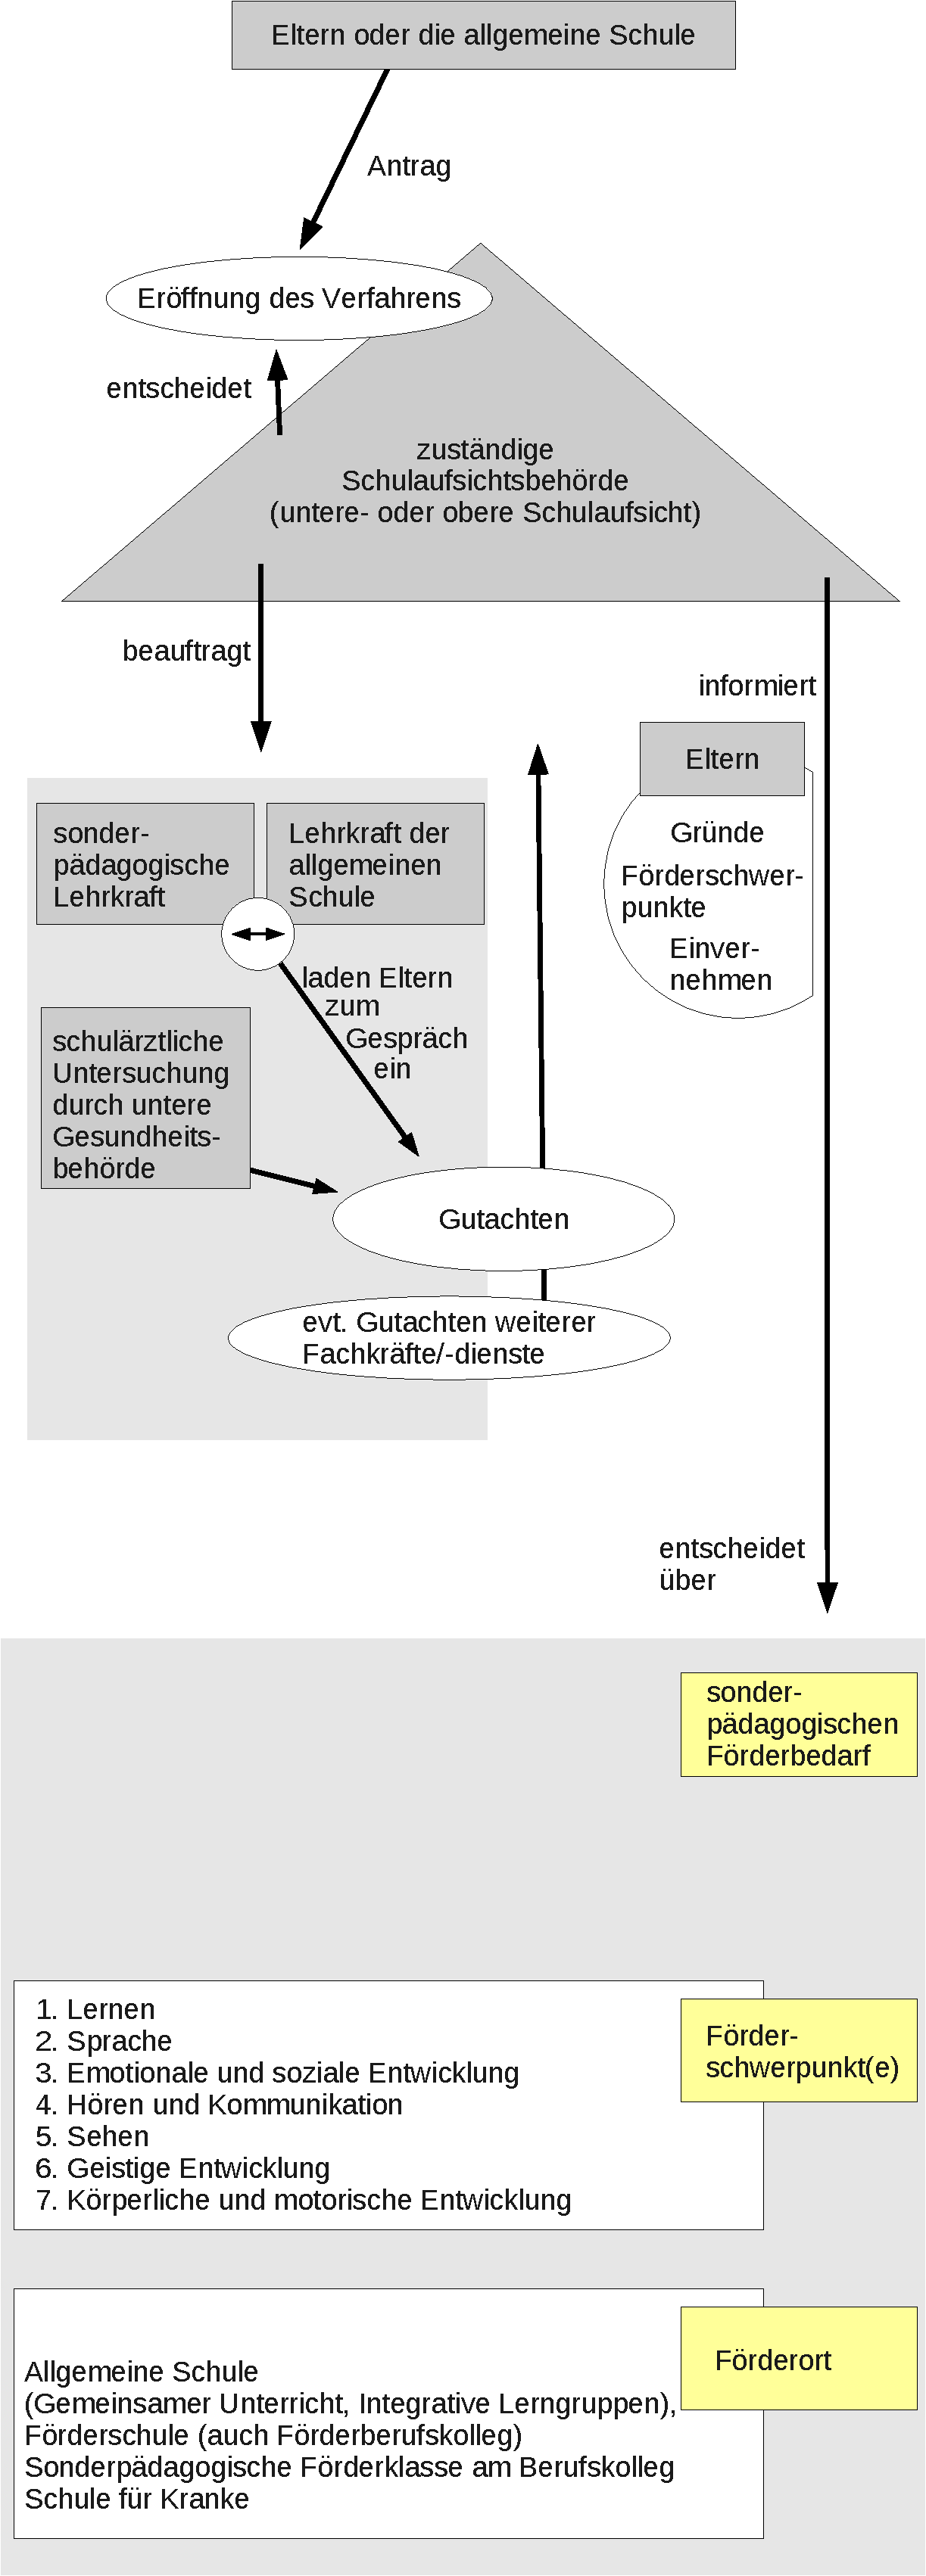
\includegraphics[width=\ScaleIfNeeded]{AO-SF.pdf}%
\caption{AO-SF Verfahren}%
\label{AO-SF Verfahren}
\end{figure}
%%%
Laut Schulgesetz des Landes NRW können Schüler sonder­päda­go­gisch gefördert werden, wenn sie
\Quelle{...
wegen ihrer körperlichen, seelischen oder geistigen Behinderung oder wegen ihres erheblich beeinträchtigten Lernvermögens nicht am Unterricht einer allgemeinen Schule (allgemein bildende oder berufsbildende Schule) teilnehmen können.}
Dies wird in einem speziellen Verfahren, dem Verfahren zur Er­mitt­lung des sonder­päda­go­gi­schen Förder­bedarfes und zur Entscheidung über den Förder­bedarf, den Förderschwerpunkt und den Förderort (s. Abbildung \ref{AO-SF Verfahren}) festgelegt. Eine \hyperlink{Behi}{Behinderung}, nach \citep{AOSF:05}, die eine sonder­pädagogische Förderung der Schüler bedingen kann, ist eine
\Quelle{
\begin{enumerate}
\item Lern- und Entwicklungsstörungen (Lernbehinderung, Sprachbehinderung, Erziehungsschwierigkeit)
\item Geistige Behinderung,
\item Körperbehinderung,
\item Hörschädigungen (Gehörlosigkeit, Schwer­hörigkeit),
\item Sehschädigungen (Blindheit, Seh­behinderung),
\item Autismus.
\end{enumerate}
}
Die, den Behinderungen entsprechenden, Förder­schwerpunkte sind in der Abbildung \ref{AO-SF Verfahren} aufge­führt. Die nicht aufgeführten Behinderten und die Schüler deren Verfahren nicht eröffnet oder negativ beschieden wurde, werden in der allgemeinen Schule unterrichtet.
Das Verfahren ist äußerst Komplex, letztendlich führt ein festgestellter sonderpädagogischer Förderbedarf zur einer dramatisch verbesserten Lehrer/Schüler Relation. Ein großer Teil des festgestellten Förderbedarfs betrifft den Förderschwerpunkt Lernen. Dieser Förderschwerpunkt ist nach meinem Kenntnisstand in dieser Form weltweit einmalig und auch in einem Sonderschulsstem nicht nachvollziehbar. 
Inklusive Bildung im Sinne der Behindertenrechtskonvention, \cite{UNCo:06}, findet in NRW nicht statt.
%%%
\section{Zahlen für NRW}
Die Daten zu den Abbildungen sind den Quellen \citeyear{MSW:01, MSW:02, MSW:03, MSW:04, MSW:05, MSW:06, MSW:07, MSW:08, MSW:09, MSW:10}
entnommen. Die Entwicklung der Gesamtschülerzahlen, der Schülerzahlen am Berufskolleg und der Zahl der Förderschüler zeigt Abbildung \ref{NRW01} (Die Zahlen in Abbildung \ref{NRW01} sind aus Gründen der Anschaulichkeit auf volle Tausend gerundet, die berechneten Zahlen werden aus den tatsächlich erhobenen Daten gewonnen).

\begin{figure}[htbp]
\centering
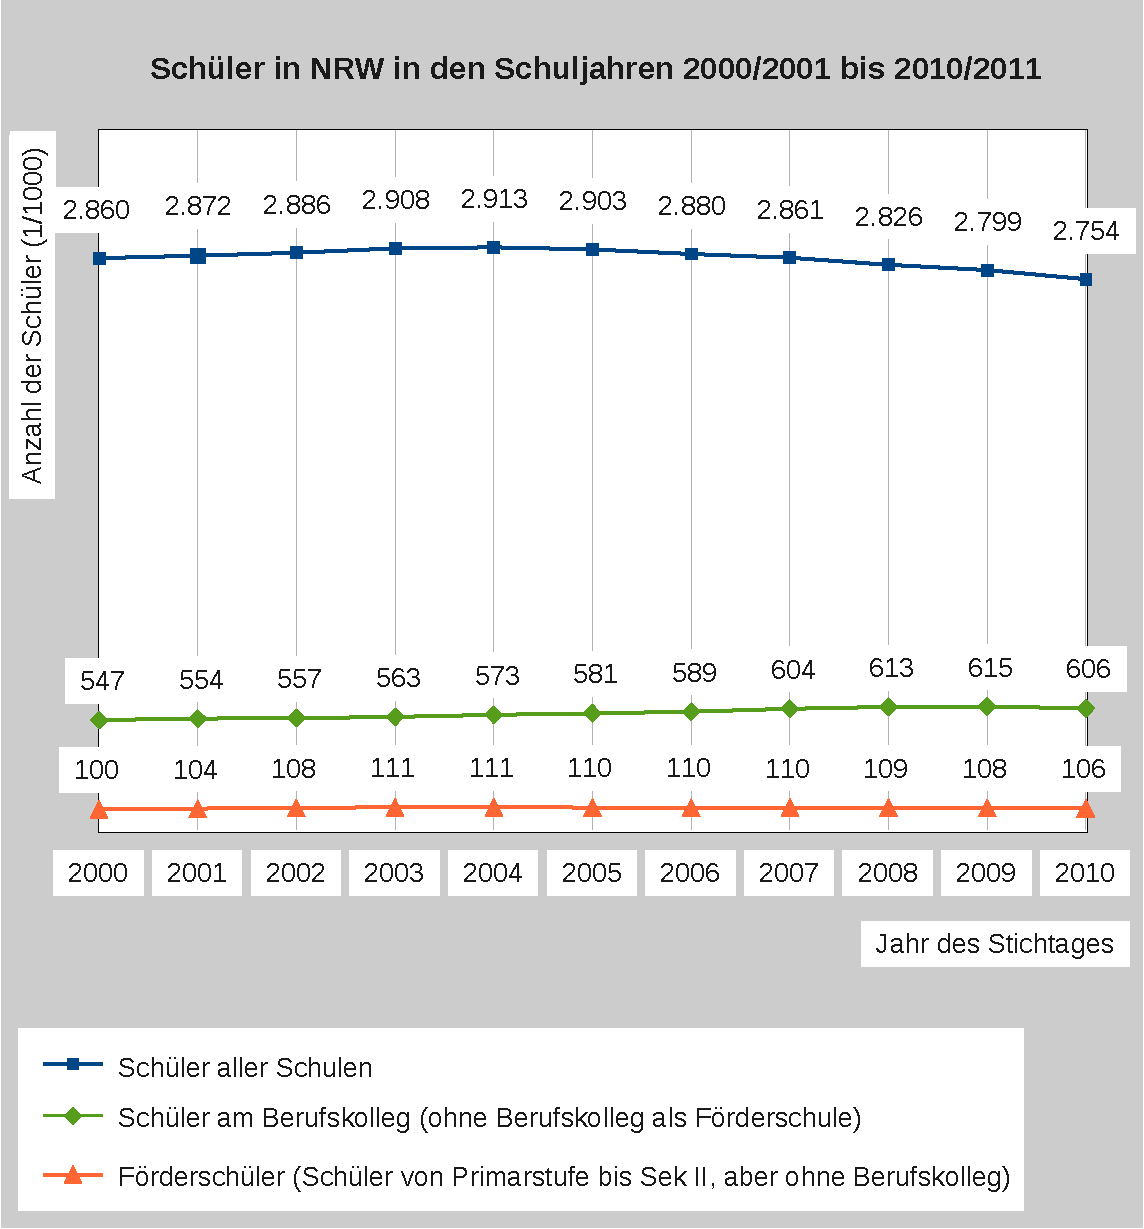
\includegraphics[width=\ScaleIfNeeded]{nrw01.pdf}%
\caption{Schüler in NRW}%
\label{NRW01}
\end{figure}
Die Förder­quote in NRW über alle Schüler (hier auch über alle Schul­be­suchs­jahre, die KMK berechnet die Förderquote nur von Klasse 1 bis 10, s. \citep{KMK:10b}) lag im Jahr 2000 bei 3,5\% und im Jahr 2010 bei 3,81\%.
Durch den de­mo­graphischen Wandel steigt im Verhältnis zur Gesamt­schüler­zahl die Zahl der Schüler am Berufs­kolleg um 2,86\% (von 19,13\% auf 21.99\%).

\begin{figure}[htbp]
\centering
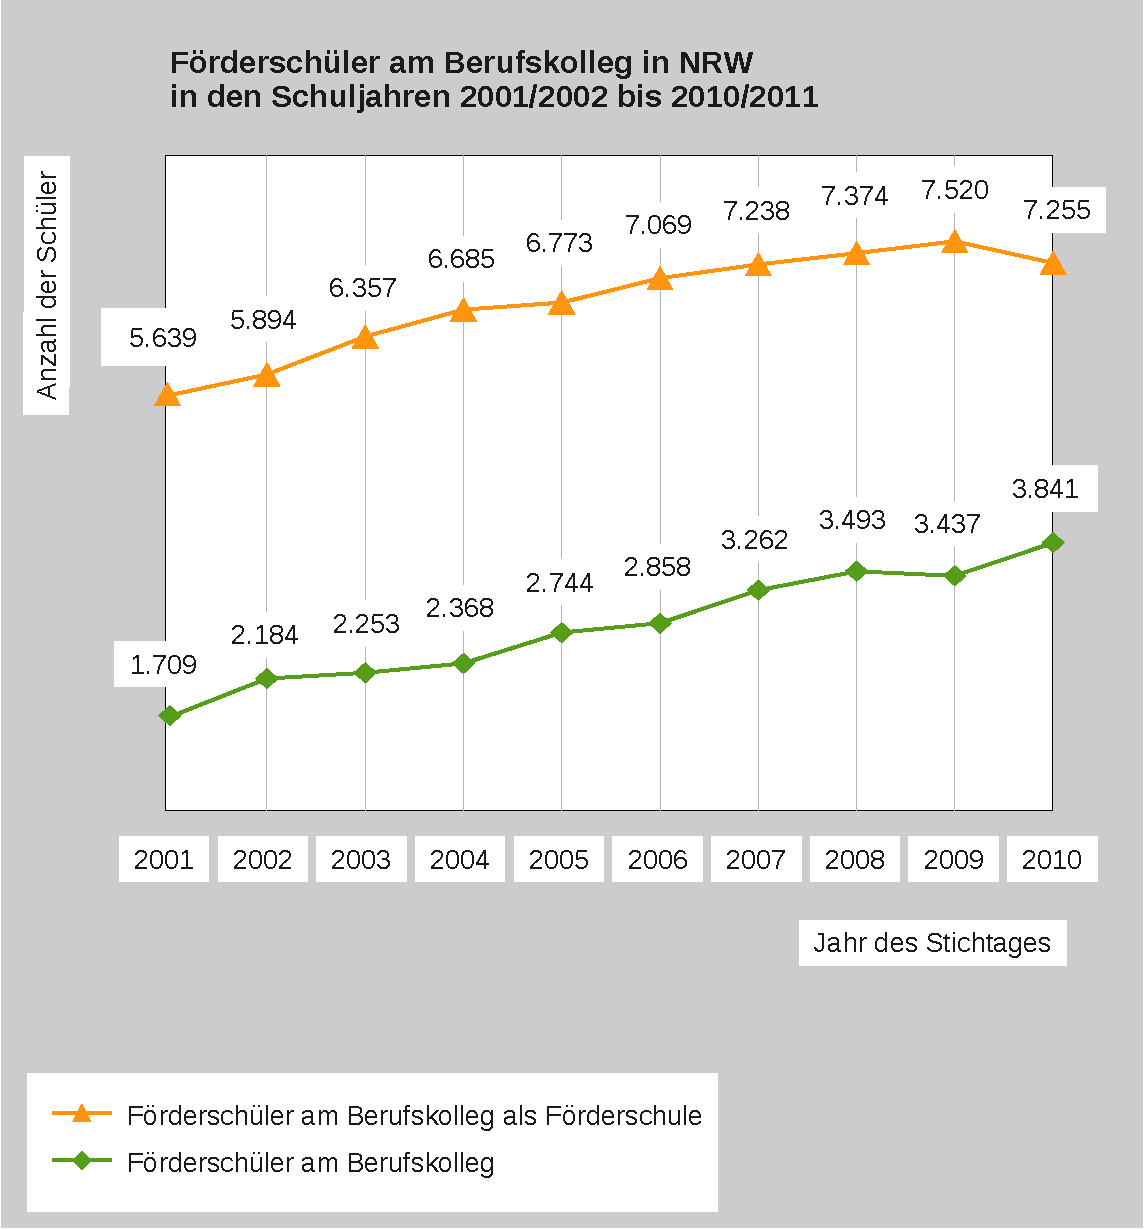
\includegraphics[width=\ScaleIfNeeded]{nrw02.pdf}%
\caption{Förderschüler am Berufskolleg}%
\label{NRW02}
\end{figure}

Von 2001 bis 2010 (hier zum Vergleich mit den Daten zum Berufskolleg von 2001 bis 2010) steigt die Förder­quote über alle Schüler um 0,21\%.\\
Die Förderschülerzahlen am Berufs­kolleg, im Zeitraum 2001 bis 2010, zeigt Abbildung \ref{NRW02}. Am Förderberufs­kolleg stieg die Förderquote um 0,18\%, am Berufs­kolleg um 0,32\% (hier ist die Förderquote bezogen auf den Anteil der Förderschüler der Berufskollegs und Förderberufskollegs zur Gesantzahl der Schüler am Berufskolleg einschließlich Förderberufskolleg). Der Anstieg der Förderquote von Förderberufskolleg und Gesamtförderquote entsprechen einander. Die Zahl der Förderschüler am Berufskolleg nimmt vergleichsweise stark zu, daraus lässt sich der politische Wille die Förderung in die Regelschule zu verlagern ablesen.

\begin{figure}[htbp]
\centering
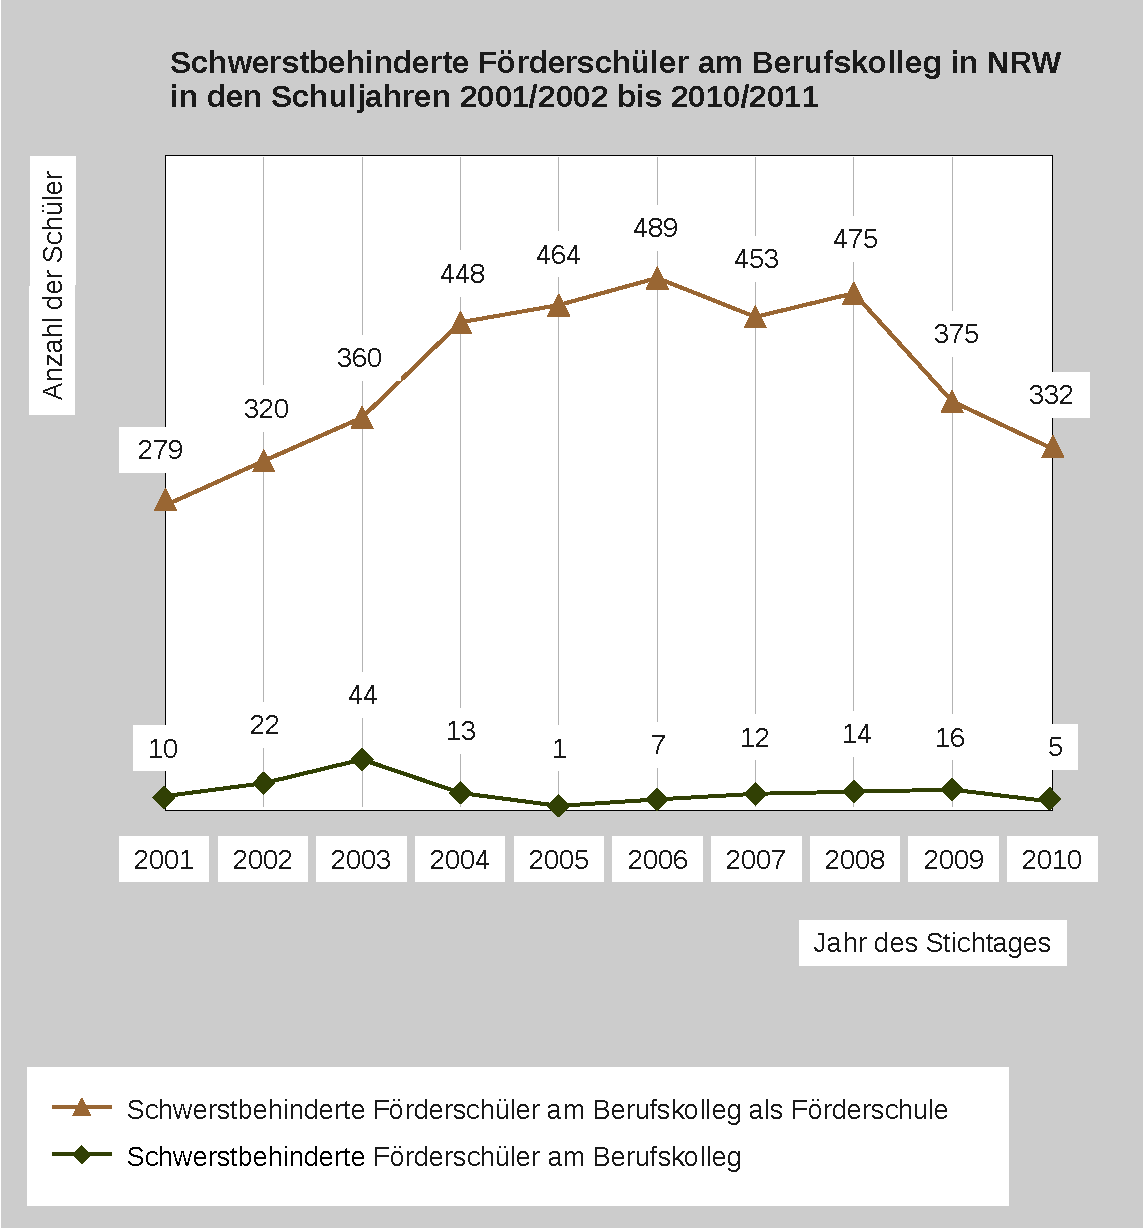
\includegraphics[width=\ScaleIfNeeded]{nrw03.pdf}%
\caption{Schwerstbehinderte Förderschüler am Berufskolleg}%
\label{NRW03}
\end{figure}

Aus den Daten zum Berufskolleg (s. Abbildungen \ref{NRW01} und \ref{NRW02}) ergibt sich für das Jahr 2001 eine Förderquote von 1,36\% und für 2010 eine Quote von 1,81\%.  Die Gesamt­förder­quote am Berufskolleg steigt damit um 0,45\%. Die Förderquote der schwerstbehinderten Schüler (s. Abbildung \ref{NRW03}) ist zu vernachlässigen. Es ist jedoch bei den schwerst­behinderten Schülern am Förder­berufs­kolleg eindeutig ein Wendepunkt im Jahr 2006 zu verzeichnen, auch hier lässt sich ein politischer Wille ablesen, der sich zumindest mit meinen Erfahrungen an einem Förderberufskolleg wiederfindet. Die Beschulung von Schwerstbehinderten am Regelberufskolleg wie sie in Abbildung \ref{NRW03} zu sehen ist halte ich für sehr unwahrscheinlich. Laut \citep{AOSF:05} ist eine Schwerbehinderung bei Schülern gegeben, wenn 
\Quelle{... geistige Behinderung, Körperbehinderung oder Erziehungsschwierigkeit erheblich über die üblichen Erscheinungsfor­men hinausgeht oder
[...] zwei oder mehr der Behinderungen Blindheit, Gehörlo­sigkeit, anhaltend hochgradige Erziehungsschwierigkeit, geistige Behinderung und hochgradige Körperbehinderung vorliegen. ...}
Es ist davon Auszugehen, dass eine Schwerbehinderung im Sinne des SGB IX in der Schulstatistik angegeben wurde. Tatsächlich sind die Begriffe Schwerbehinderung und Schwerstbehinderung nach SGB und AO-SF nicht äquivalent. Demnach berechtigt eine ausgewiesene Schwerbehinderung nach SGB nicht zu einer sonderpädgogischen Förderung nach §10 AO-SF. Die mehrfache Besetzung des Begriffes \hypertarget{Behi}{Behinderung}, kann -noch weniger nachvollziehbar-, dazu führen das ein Verfahren nicht eröffnet oder nicht positiv beschieden wird.


%\nocite{*} % Quellen im Text nicht anzeigen und alle QQuellen im Literaturverzeichnis aufführen
\bibliographystyle{natdin}
\bibliography{nore}
% bibtex
\end{document}



